%% LyX 2.2.3 created this file.  For more info, see http://www.lyx.org/.
%% Do not edit unless you really know what you are doing.
\documentclass[oneside,english]{extbook}
\usepackage{lmodern}
\renewcommand{\sfdefault}{lmss}
\renewcommand{\ttdefault}{lmtt}
\usepackage[T1]{fontenc}
\usepackage[latin9]{inputenc}
\usepackage{geometry}
\geometry{verbose,tmargin=25mm,bmargin=25mm,lmargin=25mm,rmargin=25mm}
\pagestyle{empty}
\setcounter{secnumdepth}{3}
\setcounter{tocdepth}{3}
\setlength{\parindent}{0bp}
\usepackage{babel}
\usepackage{float}
\usepackage{graphicx}
\usepackage{setspace}
\onehalfspacing
\usepackage[unicode=true,pdfusetitle,
 bookmarks=true,bookmarksnumbered=false,bookmarksopen=false,
 breaklinks=false,pdfborder={0 0 1},backref=false,colorlinks=false]
 {hyperref}

\makeatletter
%%%%%%%%%%%%%%%%%%%%%%%%%%%%%% User specified LaTeX commands.
\usepackage{amssymb}
\usepackage{color}
\usepackage{listings}
\definecolor{hellgelb}{rgb}{1,1,0.85}
\definecolor{colKeys}{rgb}{0,0,1}
\definecolor{colIdentifier}{rgb}{0,0,0}
\definecolor{colComments}{rgb}{1,0,0}
\definecolor{colString}{rgb}{0,0.5,0}
\lstset{
      language=Matlab,
      float=hbp,
      basicstyle=\footnotesize\ttfamily,
      identifierstyle=\color{colIdentifier},
      keywordstyle=\color{colKeys},
      stringstyle=\color{colString},
      commentstyle=\itshape\color{colComments},
      columns=fixed,
      tabsize=4,
      frame=single,
      framerule=1pt,
      extendedchars=true,
      showspaces=false,
      showstringspaces=false,
      numbers=left,
      numberstyle=\tiny\ttfamily,
      numbersep=1em,
      breaklines=true,
      breakindent=10pt,
      backgroundcolor=\color{hellgelb},
      breakautoindent=true,
      captionpos=t,
      xleftmargin=1em,
      xrightmargin=\fboxsep
}
\usepackage{lscape}
\usepackage{amsmath}
\usepackage{mathtools}

\makeatother

\usepackage{listings}
\renewcommand{\lstlistingname}{Listing}

\begin{document}
\renewcommand{\chaptername}{}
\renewcommand{\thechapter}{}
\pagenumbering{gobble}

\chapter{L03: FILTERING}

A discrete probability distribution satisfies:

\begin{align*}
0\,\leq\, P\left(x\right)\,\leq\, 1
\end{align*}
\begin{align*}
\sum_{x\,=\,-\infty}^{+\infty} P\left(x\right)\, =\, 1
\end{align*}

\begin{figure}[H]
\centering\includegraphics[scale=0.95]{../FIGURES/fig02}
\end{figure}

\begin{figure}[H]
\centering\includegraphics[scale=0.95]{../FIGURES/fig03}
\end{figure}

\begin{align*}
P\left(A,\,B\right)\, &=�\, P\left(B,\,A\right)\\
P\left(A,\,B\right)\, &=\,P\left(A\,|\,B\right)\,\cdot\,P\left(B\right)\\
P\left(B,\,A\right)\, &=\,P\left(B\,|\,A\right)\,\cdot\,P\left(A\right)\\
P\left(A\,|\,B\right)\,\cdot\,P\left(B\right)\, &=\, P\left(B\,|\,A\right)\,\cdot\,P\left(A\right)\\
\frac{P\left(A\,|\,B\right)}{P\left(B\,|\,A\right)}\, &=\,\frac{P\left(A\right)}{P\left(B\right)}
\end{align*}

\begin{align*}
P\left(A\right) &=\sum_{B\, =\, -\infty}^{\infty} P\left(A,\,B\right)\, =\,\sum_{B\, =\, -\infty}^{\infty} P\left(A\,|\,B\right)\,\cdot\,P\left(B\right)\\ P\left(B\right) &=\sum_{A\, =\, -\infty}^{\infty} P\left(B,\,A\right)\, =\,\sum_{A\, =\, -\infty}^{\infty} P\left(B\,|\,A\right)\,\cdot\,P\left(A\right)
\end{align*}

\begin{align*}
P\left(99\right) &=\sum_{A\, =\, -\infty}^{\infty} P\left(99, A\right) = P\left(99, 0\right) = P\left(99\,|\,0\right)\cdot P\left(0\right) = 0.25\cdot 1.00 = 25\\ P\left(100\right) &=\sum_{A\, =\, -\infty}^{\infty} P\left(100, A\right) = P\left(100, 0\right) = P\left(100\,|\,0\right)\cdot P\left(0\right) = 0.50\cdot 1.00 = 0.50\\ P\left(101\right) &=\sum_{A\, =\, -\infty}^{\infty} P\left(101, A\right) = P\left(101, 0\right) = P\left(101\,|\,0\right)\cdot P\left(0\right) = 0.25\cdot 1.00 = 0.25
\end{align*}

\begin{align*}
P\left(198,\,99\right)\,&=\,P\left(198\,|\,99\right)\,\cdot\,P\left(99\right)\,=\,0.25\,\cdot\,0.25\,=\,0.0625\\ P\left(199,\,99\right)\,&=\,P\left(199\,|\,99\right)\,\cdot\,P\left(99\right)\,=\,0.50\,\cdot\,0.25\,=\,0.1250\\ P\left(200,\,99\right)\,&=\,P\left(200\,|\,99\right)\,\cdot\,P\left(99\right)\,=\,0.25\,\cdot\,0.25\,=\,0.0625\\ P\left(199,\,100\right)\,&=\,P\left(199\,|\,100\right)\,\cdot\,P\left(100\right)\,=\,0.25\,\cdot\,0.50\,=\,0.1250\\ P\left(200,\,100\right)\,&=\,P\left(200\,|\,100\right)\,\cdot\,P\left(100\right)\,=\,0.50\,\cdot\,0.50\,=\,0.2500\\ P\left(201,\,100\right)\,&=\,P\left(201\,|\,100\right)\,\cdot\,P\left(100\right)\,=\,0.25\,\cdot\,0.50\,=\,0.1250\\ P\left(200,\,101\right)\,&=\,P\left(200\,|\,101\right)\,\cdot\,P\left(101\right)\,=\,0.25\,\cdot\,0.25\,=\,0.0625\\ P\left(201,\,101\right)\,&=\,P\left(201\,|\,101\right)\,\cdot\,P\left(101\right)\,=\,0.50\,\cdot\,0.25\,=\,0.1250\\ P\left(202,\,101\right)\,&=\,P\left(202\,|\,101\right)\,\cdot\,P\left(101\right)\,=\,0.25\,\cdot\,0.25\,=\,0.0625
\end{align*}

\begin{align*}
P\left(198\right)\,&=\,P\left(198,\,99\right)\,=\,0.0625\\ P\left(199\right)\,&=\,P\left(199,\,99\right)\,+\,P\left(199,\,100\right)\,=\,0.1250\,+\,0.1250\,=\,0.2500\\ P\left(200\right)\,&=\,P\left(200,\,99\right)\,+\,P\left(200,\,100\right)\,+\,P\left(200,\,101\right)\,=\,0.0625\,+\,0.2500\,+\,0.0625\,=\,0.3750\\ P\left(201\right)\,&=\,P\left(201,\,100\right)\,+\,P\left(201,\,101\right)\,=\,0.1250\,+\,0.1250\,=\,0.2500\\ P\left(202\right)\,&=\,P\left(202,\,101\right)\,=\,0.0625
\end{align*}

\begin{figure}[H]
\centering\includegraphics[scale=0.95]{../FIGURES/fig05}
\end{figure}

\begin{figure}[H]
\centering\includegraphics[scale=0.95]{../FIGURES/fig06}
\end{figure}

\begin{figure}[H]
\centering\includegraphics[scale=0.95]{../FIGURES/fig07}
\end{figure}

A discrete probability distribution can be calculated using a discrete
convolution operation:

\begin{align*}
P\left[B\right]\,=\,(f\,*\,g)\left[B\right]\,=\,\sum_{A\,=\,-\infty}^{\infty} f\left[B\,-\,A\right]\,\cdot\,g\left[A\right]
\end{align*}

\begin{figure}[H]
\includegraphics[scale=0.95]{../FIGURES/fig09}
\end{figure}

\begin{align*}
P\left[B\right]&\,=\,f\left[B\,-\,\left(-\infty\right)\right]\,\cdot\,g\left[-\infty\right]\,+\,\ldots\,+\,f\left[B\,-\,9\right]\,\cdot\,g\left[9\right]\,+\,\\ &\,+\,f\left[B\,-\,10\right]\,\cdot\,g\left[10\right]\,+\,f\left[B\,-\,11\right]\,\cdot\,g\left[11\right]\,+\,f\left[B\,-\,12\right]\,\cdot\,g\left[12\right]\,+\,f\left[B\,-\,13\right]\,\cdot\,g\left[13\right]\,+\,\\ &\,+\,f\left[B\,-\,14\right]\,\cdot\,g\left[14\right]\,+\,\ldots\,+\,f\left[B\,-\,\infty\right]\,\cdot\,g\left[\infty\right]
\end{align*}\\

$g\left[\,\cdot\,\right]\, =\, 0$ for$A\, =\, (-\infty,\, 9]\,\cup\, [14,\,\infty)$

The first non-zero value of the function$g\left[\,\cdot\,\right]$
appears at$A\, =\, 10$,$g\left[10\right]\, =\, 0.25$, and the last
non-zero value appears at$A\, =\, 13$,$g\left[13\right]\, =\, 0.125$\\

The first non-zero value of the function$f\left[\,\cdot\,\right]$
appears at:

\[
B\, -\, 10\, =\, 5\,\rightarrow\, B\, =\, 15
\]and the last non-zero value appears at

\[
B\, -\, 13\, =\, 7\,\rightarrow\, B\, =\, 20
\]\\
The length of the discrete probability distribution$P\left[B\right]$
is

\[
N\, +\, M\, -\, 1\, =\, 3\, +\, 4\, -\, 1\, =\, 6
\]The first non-zero value of$P\left[B\right]$ is\\
\begin{center}
\texttt{first n where $g\left[ n\right]\,\neq\, 0\, +$ first m where $f\left[ m\right]\,\neq\, 0$}
\[
5\, +\, 10\, =\, 15
\]
\par\end{center}

The last non-zero value of$P\left[B\right]$ is\\
\begin{center}
\texttt{last n where $g\left[ n\right]\,\neq\, 0\, +$ last m where $f\left[ m\right]\,\neq\, 0$}
\[
7\, +\, 13\, =\, 20
\]
\par\end{center}

or alternatively\\
\begin{center}
\texttt{The first non-zero value of $P\left[ B\right]\, +\, length\left( P\left[ B\right]\right)\, -\, 1$}
\[
15\, +\, 6\, -\, 1\, =\, 20
\]
\par\end{center}

Graphical calculation of the convolution operation:

\begin{figure}[H]
\centering\includegraphics[scale=0.95]{../FIGURES/fig11}
\end{figure}

\begin{align*}
P\left[B\right]\,=\,(f\,*\,g)\left[B\right]\,=\,\sum_{A\,=\,-\infty}^{\infty} f\left[B\,-\,A\right]\,\cdot\,g\left[A\right]
\end{align*}

\begin{figure}[H]
\centering\includegraphics[scale=0.95]{../FIGURES/fig13}
\end{figure}

\begin{lstlisting}
Pseudo-code to compute a discrete convolution:
total_length = len(f.values) + len(g.values) - 1
P = [0] * total_length
fsp = f.start_pos # Position of the first non-zero value in f.values
gsp = g.start_pos # Position of the first non-zero value in g.values
psp = tsp + gsp    # Position of the first non-zero value in P.values
for i in xrange(0, total_length): #From 0 to total_length-1
    for j in xrange(i, -1, -1):   #From i to 0
        P[i] += f.values[i -j] * g.values[j]
\end{lstlisting}

\begin{figure}[H]
\centering\includegraphics[scale=0.68]{../FIGURES/fig14}
\end{figure}

\begin{figure}[H]
\centering\includegraphics{../FIGURES/fig16}
\end{figure}

\begin{align*}
p\left(x\, |\, z\right)\, =\,\frac{p\left(z\, |\, x\right)\,\cdot\, p\left(x\right)}{p\left(z\right)}\, =\,\frac{p\left(z\, |\, x\right)\,\cdot\, p\left(x\right)}{\sum_{\tau\, =\, -\infty}^{+\infty}p\left(z,\,\tau\right)}\, =\,\frac{p\left(z\, |\, x\right)\,\cdot\, p\left(x\right)}{\sum_{\tau\, =\, -\infty}^{+\infty}p\left(z\, |\,\tau\right)\,\cdot\, p\left(\tau\right)}\, =\,\alpha\,\cdot\, p\left(z\, |\, x\right)\,\cdot\, p\left(x\right)
\end{align*}

\begin{figure}[H]
\centering\includegraphics{../FIGURES/fig17}
\end{figure}

\begin{figure}[H]
\centering\includegraphics[scale=0.8]{../FIGURES/fig19}
\end{figure}

\begin{figure}[H]
\centering\includegraphics[scale=0.9]{../FIGURES/fig20}
\end{figure}
\begin{center}
\textbf{Motion - Convolution}
\par\end{center}

\begin{align*}
p\left( x\right)\, =\,\sum_{y\, =\, -\infty}^{+\infty}  p\left( x,\, y\right)\, =\,\sum_{y\, =\, -\infty}^{+\infty}  p\left( x\, |\, y\right)\,\cdot\, p\left(y\right)
\end{align*}\\
\begin{center}
\textbf{Measurement - Multiplication}
\par\end{center}

\begin{align*}
p\left(x\, |\, z\right)\, =\,\alpha\,\cdot\, p\left(z\, |\, x\right)\,\cdot\, p\left(x\right)
\end{align*}\\
\begin{center}
\textbf{THE BAYES FILTER IN 1 DIMENSION}
\par\end{center}

\begin{figure}[H]
\centering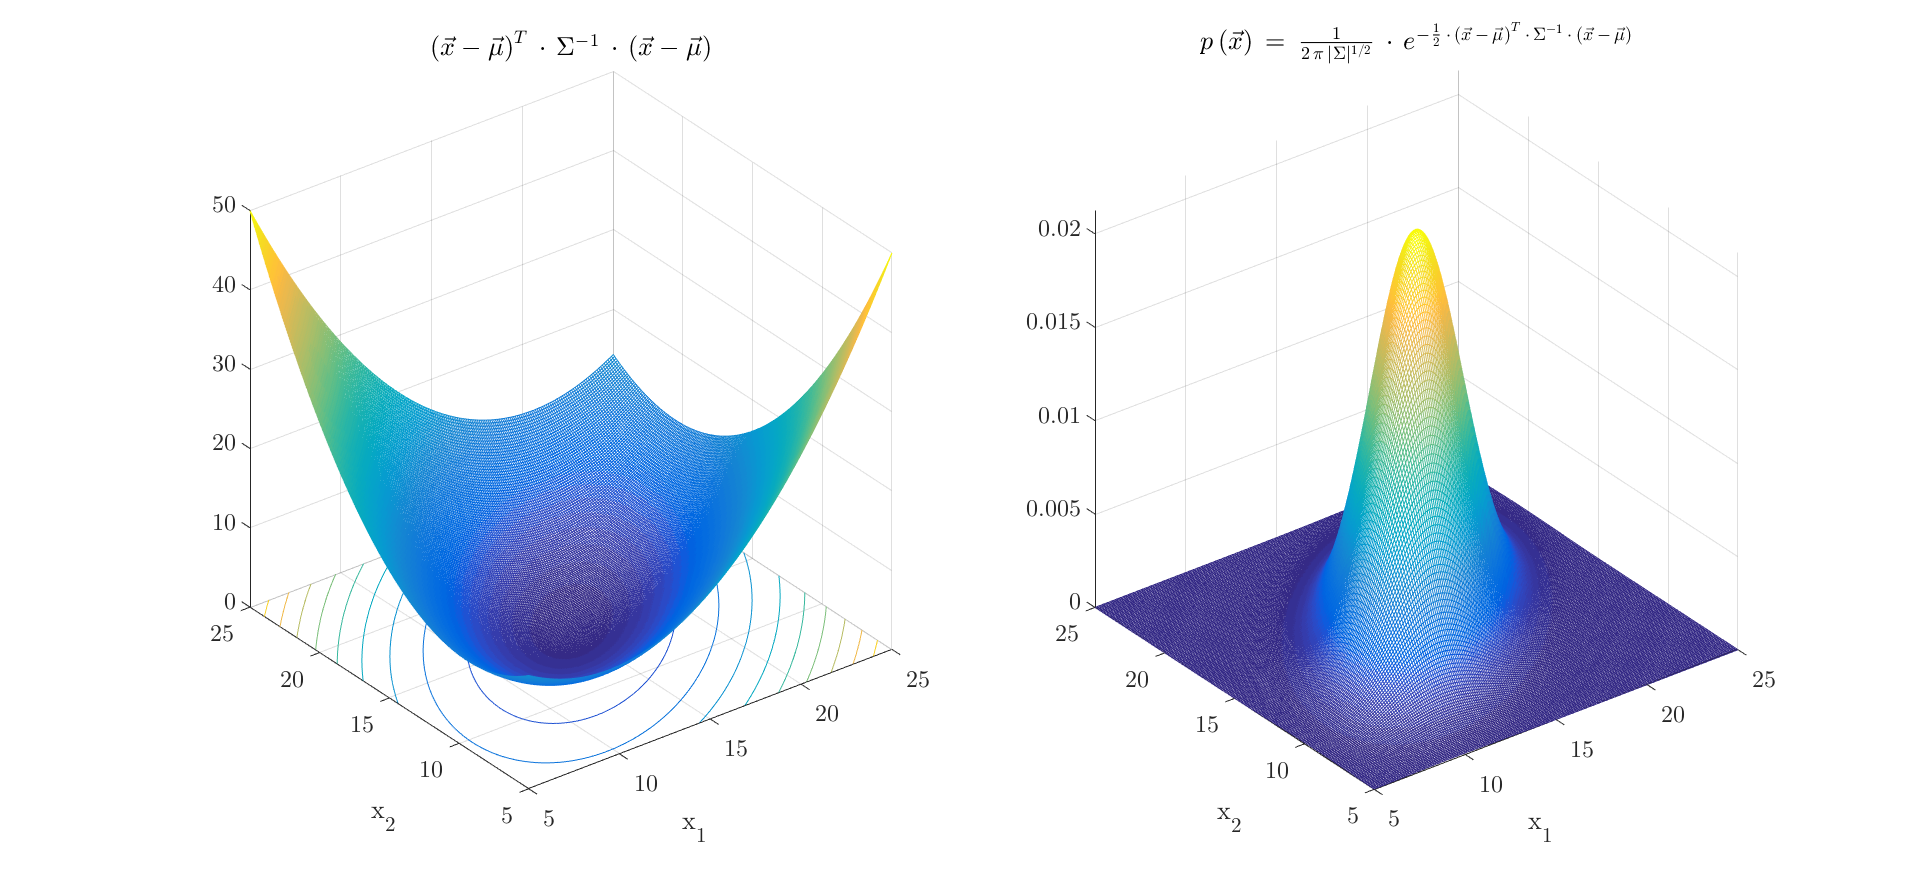
\includegraphics[scale=0.95]{../FIGURES/fig21}
\end{figure}

Belief with bar,$\overline{bel}\left(x_t\right)$: after the robot
has moved and before the robot takes measurements:

\begin{align*}
p\left(x_t\, |\, u_t,\, z_{t-1}\right)\, =\, &\int_{x_{t-1}\, =\, -\infty}^{+\infty} p\left(x_t,\, x_{t-1}\, |\, u_t,\, z_{t-1}\right)\, dx_{t-1}\, =\,\\
=\, &\int_{x_{t-1}\, =\, -\infty}^{+\infty} p\left(x_t\, |\, x_{t-1},\, u_t,\, z_{t-1}\right)\,\cdot\, p\left(x_{t-1}\, |\, u_t,\, z_{t-1}\right)\, dx_{t-1}
\end{align*}

\begin{align*}
p\left(x_t\, |\, u_t,\, z_{t-1}\right)\, &\longrightarrow\, p\left(x_t\right)\\
p\left(x_t\, |\, x_{t-1},\, u_t,\, z_{t-1}\right)\, &\longrightarrow\, p\left(x_t\, |\, x_{t-1},\, u_t\right)\\
p\left(x_{t-1}\, |\, u_t,\, z_{t-1}\right)\, &\longrightarrow\, p\left(x_{t-1}\, |\, z_{t-1}\right)
\end{align*}

\begin{align*}
\overline{bel}\left(x_{t}\right)\, &=\, p\left(x_t\right)\\
bel\left(x_{t-1}\right)\, &=\, p\left(x_{t-1}\, |\, z_{t-1}\right)
\end{align*}

\begin{align*}
\overline{bel}\left(x_t\right)\, =\,\int_{x_{t-1}\, =\, -\infty}^{+\infty} p\left(x_t\, |\, x_{t-1},\, u_t\right)\,\cdot\, bel\left(x_{t-1}\right)\, dx_{t-1}
\end{align*}

Belief without bar,$bel\left(x_t\right)$: after the robot has moved
and after the robot has taken measurements:

\begin{align*}
bel\left(x_t\right)\, =\, p\left(x_t\, |\, z_t\right)\, =\,\frac{p\left(z_t\, |\, x_t\right)\,\cdot\, p\left(x_t\right)}{p\left(z_t\right)}\, =\,\alpha\,\cdot\, p\left(z_t\, |\, x_t\right)\,\cdot\,\overline{bel}\left(x_t\right)
\end{align*}\\
\begin{itemize}
\item \textbf{INPUT:}$bel\left(x_{t-1}\right),\, u_t,\, z_t$
\item \textbf{OUTPUT:}$bel\left(x_t\right)$
\end{itemize}
Normal distribution:

\begin{align*}
v\,\sim\,\mathcal{N}(v,\,\mu,\,\sigma^{2})\, =\,\frac{1}{\sigma\sqrt{2\pi}}\, e^{-\frac{1}{2}\left(\frac{v\, -\,\mu}{\sigma}\right)^2}
\end{align*}

\begin{figure}[H]
\centering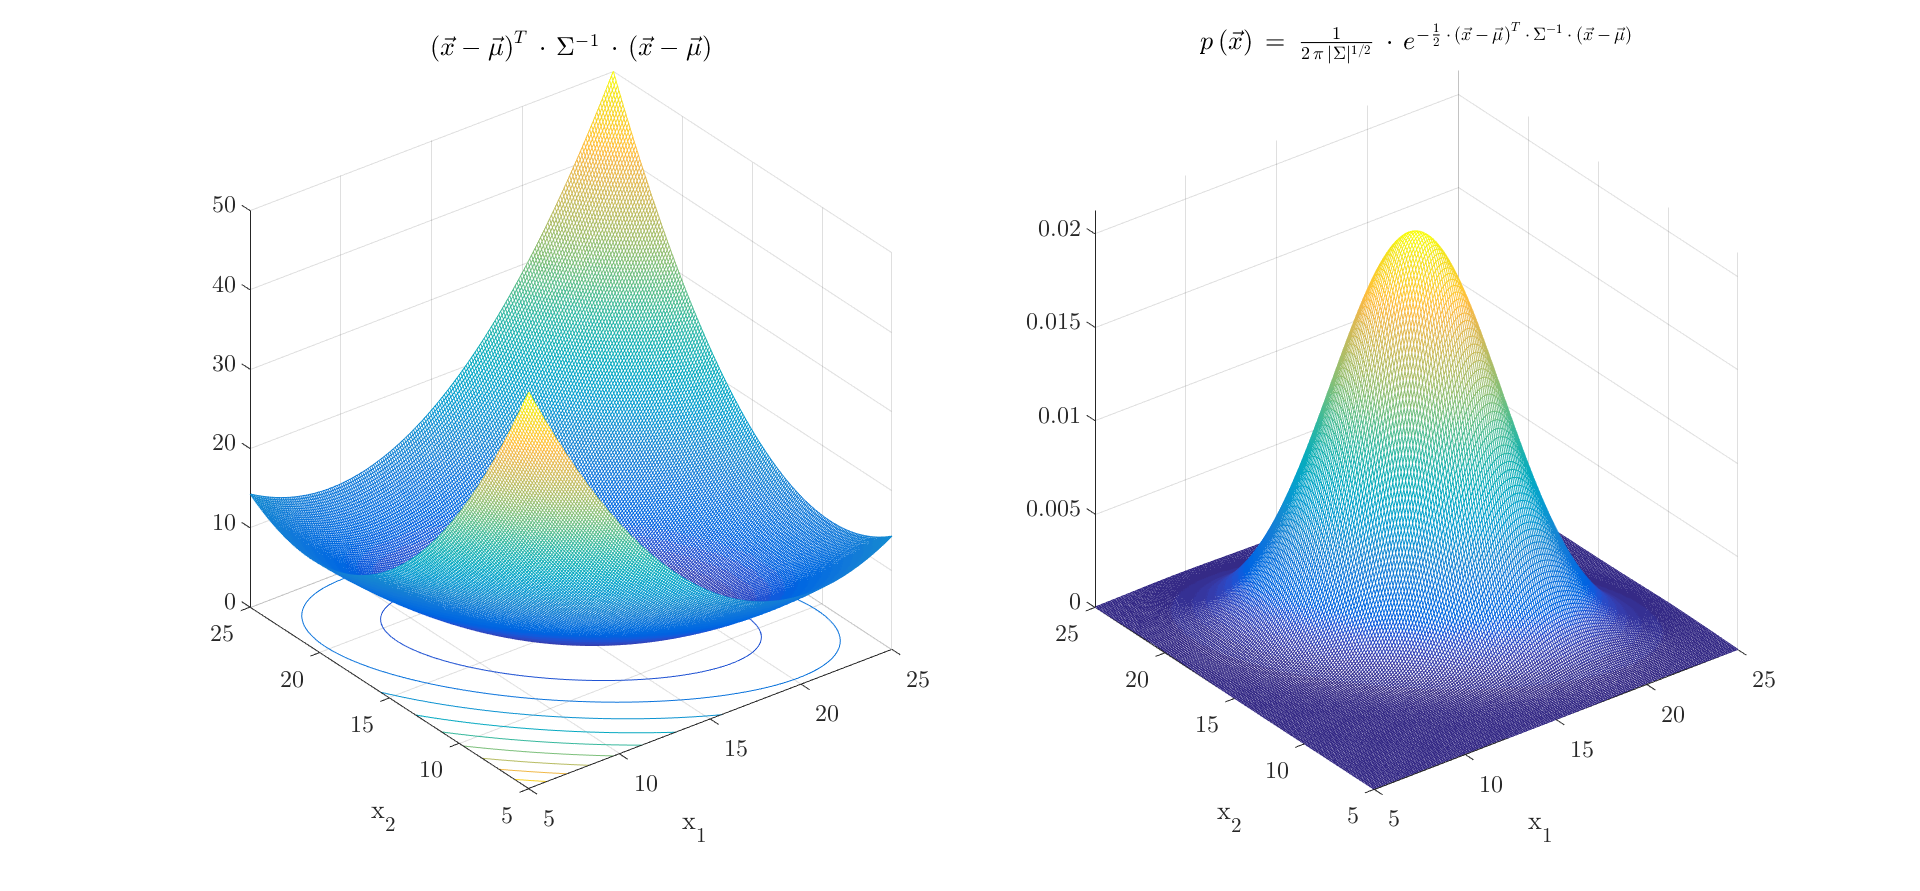
\includegraphics[scale=0.95]{../FIGURES/fig23}
\end{figure}

\begin{align*}
z_t\, &=\, c_t\,\cdot\, x_t\, +\,\epsilon_{Q_t}\\
p\left(\epsilon_{Q_t}\right)\, &=\,\mathcal{N}\left(0,\,\sigma_{Q_t}^2\right)
\end{align*}

\begin{align*}
p\left(z_t\, |\, x_t\right)\, & =\,\mathcal{N}(c_t\,\cdot\, x_t,\,\sigma_{Q_t}^{2})\\
\overline{bel}\left(x_t\right)\, & =\,\mathcal{N}(\overline{\mu_t},\,\overline{\sigma_t}^2)\\
bel\left(x_t\right)\, & =\, p\left(x_t\, |\, z_t\right)\, =\\
&=\,\alpha\,\cdot\, p\left(z_t\, |\, x_t\right)\,\cdot\,\overline{bel}\left(x_t\right)\, =\\
& =\,\alpha'\,\cdot\, e^{-\frac{1}{2}\left(\frac{z_t\, -\, c_t\,\cdot\, x_t}{\sigma_{Q_t}}\right)^2}\,\cdot\, e^{-\frac{1}{2}\left(\frac{x_t\, -\,\overline{\mu_t}}{\overline{\sigma_t}}\right)^2}\, =\\
& =\,\alpha'\,\cdot\, e^{-\left(\frac{1}{2}\left(\frac{z_t\, -\, c_t\,\cdot\, x_t}{\sigma_{Q_t}}\right)^2\, +\,\frac{1}{2}\left(\frac{x_t\, -\,\overline{\mu_t}}{\overline{\sigma_t}}\right)^2\right)}\, =\\
& =\,\alpha''\,\cdot\, e^{-\frac{1}{2}\left(\frac{x_t\, -\,\mu_t}{\sigma_t}\right)^2}\, =\,\mathcal{N}(\mu_t,\,\sigma_t^{2})
\end{align*}

\begin{align*}
f\left(x\right)\, &=\,\frac{1}{2}\,\cdot\, A\,\cdot\,\left(x\, -\, B\right)^2\, +\, C\\
\frac{df\left(x\right)}{dx}\, &=\, A\,\cdot\,\left(x\, -\, B\right)\, =\, 0\,\rightarrow\, x\, =\, B\\
\frac{d^2f\left(x\right)}{dx^2}\,& =\, A
\end{align*}

\begin{align*}
f\left(x_t\right)\, &=\,\frac{1}{2}\,\cdot\, A\,\cdot\,\left(x_t\, -\, B\right)^2\, +\, C\, =\,\\
&=\,\frac{1}{2}\,\cdot\,\frac{1}{\sigma_{Q_t}^2}\,\cdot\,\left(z_t\, -\, c_t\,\cdot\, x_t\right)^2\, +\,\frac{1}{2}\,\cdot\,\frac{1}{\overline{\sigma_t}^2}\,\cdot\,\left(x_t\, -\,\overline{\mu_t}\right)^2\\
\frac{d^2f\left(x_t\right)}{dx_t^2}\, &=\, A\, =\,\frac{c_t^2}{\sigma_{Q_t}^2}\,+\,\frac{1}{\overline{\sigma_t}^2}\\
\frac{df\left(x_t\right)}{dx_t}\, &=\, A\,\cdot\,\left(x_t\, -\, B\right)\, =\,\\
&=\,\frac{1}{\sigma_{Q_t}^2}\,\cdot\,\left(z_t\, -\, c_t\,\cdot\, x_t\right)\,\cdot\,\left(-c_t\right)\, +\,\frac{1}{\overline{\sigma_t}^2}\,\cdot\,\left(x_t\, -\,\overline{\mu_t}\right)\, =\,\\
&=\, x_t\,\cdot\,\left(\frac{c_t^2}{\sigma_{Q_t}^2}\, +\,\frac{1}{\overline{\sigma_t}^2}\right)\, -\,\frac{z_t\,\cdot\, c_t}{\sigma_{Q_t}^2}\,-\,\frac{\overline{\mu_t}}{\overline{\sigma_t}^2}\, =\,0
\end{align*}

\begin{align*}
x_t\, =\, B\, =\,\frac{\frac{z_t\,\cdot\, c_t}{\sigma_{Q_t}^2}\, +\,\frac{\overline{\mu_t}}{\overline{\sigma_t}^2}}{\frac{c_t^2}{\sigma_{Q_t}^2}\, +\,\frac{1}{\overline{\sigma_t}^2}}\, =\,\frac{\frac{z_t\,\cdot\, c_t}{\sigma_{Q_t}^2}\, +\,\frac{\overline{\mu_t}}{\overline{\sigma_t}^2}}{A}
\end{align*}

\begin{align*}
\alpha'\,\cdot\, e^{-\left(\frac{1}{2}\left(\frac{z_t\, -\, c_t\,\cdot\, x_t}{\sigma_{Q_t}}\right)^2\, +\,\frac{1}{2}\left(\frac{x_t\, -\,\overline{\mu_t}}{\overline{\sigma_t}}\right)^2\right)}\, =\,\alpha'\,\cdot\, e^{-\left(\frac{1}{2}\,\cdot\, A\,\cdot\,\left(x_t\, -\, B\right)^2\, +\, C\right)}\, =\,\alpha''\,\cdot\, e^{-\frac{1}{2}\left(\frac{x_t\, -\,\mu_t}{\sigma_t}\right)^2}
\end{align*}

\begin{align*}
\alpha'\,\cdot\, e^{-\left(\frac{1}{2}\,\cdot\, A\,\cdot\,\left(x_t\, -\, B\right)^2\, +\, C\right)}\, &=\,\alpha''\,\cdot\, e^{-\frac{1}{2}\left(\frac{x_t\, -\,\mu_t}{\sigma_t}\right)^2}\\
\alpha'\,\cdot\, e^{-C}\,\cdot\, e^{-\frac{1}{2}\,\cdot\, A\,\cdot\,\left(x_t\, -\, B\right)^2}\, &=\,\alpha''\,\cdot\, e^{-\frac{1}{2}\left(\frac{x_t\, -\,\mu_t}{\sigma_t}\right)^2}
\end{align*}

\begin{align*}
\frac{1}{\sigma_t^2}\, &=\, A\\
\sigma_t^2\, &=\,\frac{1}{A}\, =\,\frac{1}{\frac{c_t^2}{\sigma_{Q_t}^2}\, +\,\frac{1}{\overline{\sigma_t}^2}}\, =\,\frac{\sigma_{Q_t}^2\,\cdot\,\overline{\sigma_t}^2}{c_t^2\,\cdot\,\overline{\sigma_t}^2\, +\,\sigma_{Q_t}^2}
\end{align*}
\begin{center}
\begin{align*}
\mu_t\, =\, B\, =\,\frac{\frac{z_t\,\cdot\, c_t}{\sigma_{Q_t}^2}\, +\,\frac{\overline{\mu_t}}{\overline{\sigma_t}^2}}{A}\, &=\,\sigma_t^2\,\cdot\,\left(\frac{z_t\,\cdot\, c_t}{\sigma_{Q_t}^2}\, +\,\frac{\overline{\mu_t}}{\overline{\sigma_t}^2}\right)\\
& =\,\sigma_t^2\,\cdot\,\left(\frac{z_t\,\cdot\, c_t}{\sigma_{Q_t}^2}\, +\,\frac{\overline{\mu_t}}{\overline{\sigma_t}^2}\right)\\
&=\,\sigma_t^2\,\cdot\,\left(\frac{c_t}{\sigma_{Q_t}^2}\,\cdot\,\left(z_t\, -\, c_t\,\overline{\mu_t}\, +\, c_t\,\overline{\mu_t}\right)\, +\,\frac{\overline{\mu_t}}{\overline{\sigma_t}^2}\right)\\
&=\,\sigma_t^2\,\cdot\,\left(\frac{c_t}{\sigma_{Q_t}^2}\,\cdot\,\left(z_t\, -\, c_t\,\overline{\mu_t}\right)\, +\,\frac{c_t^2}{\sigma_{Q_t}^2}\overline{\mu_t}\, +\,\frac{\overline{\mu_t}}{\overline{\sigma_t}^2}\right)\\
&=\,\sigma_t^2\,\cdot\,\left(\frac{c_t}{\sigma_{Q_t}^2}\,\cdot\,\left(z_t\, -\, c_t\,\overline{\mu_t}\right)\, +\,\left(\frac{c_t^2}{\sigma_{Q_t}^2}\, +\,\frac{1}{\overline{\sigma_t}^2}\right)\,\cdot\,\overline{\mu_t}\right)\\
&=\,\sigma_t^2\,\cdot\,\left(\frac{c_t}{\sigma_{Q_t}^2}\,\cdot\,\left(z_t\, -\, c_t\,\overline{\mu_t}\right)\, +\,\frac{1}{\sigma_t^2}\,\cdot\,\overline{\mu_t}\right)\\
&=\,\frac{\sigma_t^2}{\sigma_{Q_t}^2}\,\cdot\, c_t\,\cdot\,\left(z_t\, -\, c_t\,\overline{\mu_t}\right)\, +\,\overline{\mu_t}
\end{align*}\\
\textbf{KALMAN GAIN}
\par\end{center}

\begin{align*}
K_t\, &=\,\frac{\sigma_t^2}{\sigma_{Q_t}^2}\,\cdot\, c_t\\
\mu_t\, &=\,\overline{\mu_t}\, +\, K_t\,\cdot\,\left(z_t\, -\, c_t\,\overline{\mu_t}\right)
\end{align*}

where:
\begin{itemize}
\item $\mu_t$ is the estimated state (or corrected state), aka $\hat{x}_t$.
\item $\overline{\mu_t}$ is the predicted state, aka $\tilde{x}_t$.
\item $K_t$ is the Kalman gain.
\item $z_t$ is the actual measurement.
\item $c_t\,\overline{\mu_t}$ is the expected measurement.
\item $\left(z_t\, -\, c_t\,\overline{\mu_t}\right)$ is called innovation.
\end{itemize}
\begin{align*}
K_t\, =\,\frac{\sigma_t^2}{\sigma_{Q_t}^2}\,\cdot\, c_t\,=\,\frac{c_t}{\sigma_{Q_t}^2\,\cdot\,\left(\frac{c_t^2}{\sigma_{Q_t}^2}\, +\,\frac{1}{\overline{\sigma_t}^2}\right)}\, =\,\frac{c_t\,\cdot\,\overline{\sigma_t}^2}{c_t\,\cdot\,\overline{\sigma_t}^2\, +\,\sigma_{Q_t}^2}
\end{align*}\begin{align*}
\sigma_{Q_t}^2\,\,\,\uparrow\,\,\,\longrightarrow\, K_t\,\downarrow
\end{align*}\begin{align*}
K_t\, &=\,\frac{c_t\,\cdot\,\overline{\sigma_t}^2}{c_t^2\,\cdot\,\overline{\sigma_t}^2\, +\,\sigma_{Q_t}^2}\\
\mu_t\, &=\,\overline{\mu_t}\, +\, K_t\,\cdot\,\left(z_t\, -\, c_t\,\overline{\mu_t}\right)\\
\sigma_t^2\, &=\,\left(1\, -\, K_t\,\cdot\, c_t\right)\,\cdot\,\overline{\sigma_t}^2
\end{align*}\begin{align*}
K_t\, &=\, 0\,\,\longrightarrow\,\,\sigma_t^2\, =\,\overline{\sigma_t}^2\\
K_t\, &>\, 0\,\,\longrightarrow\,\,\sigma_t^2\, <\,\overline{\sigma_t}^2
\end{align*}

\begin{figure}[H]
\centering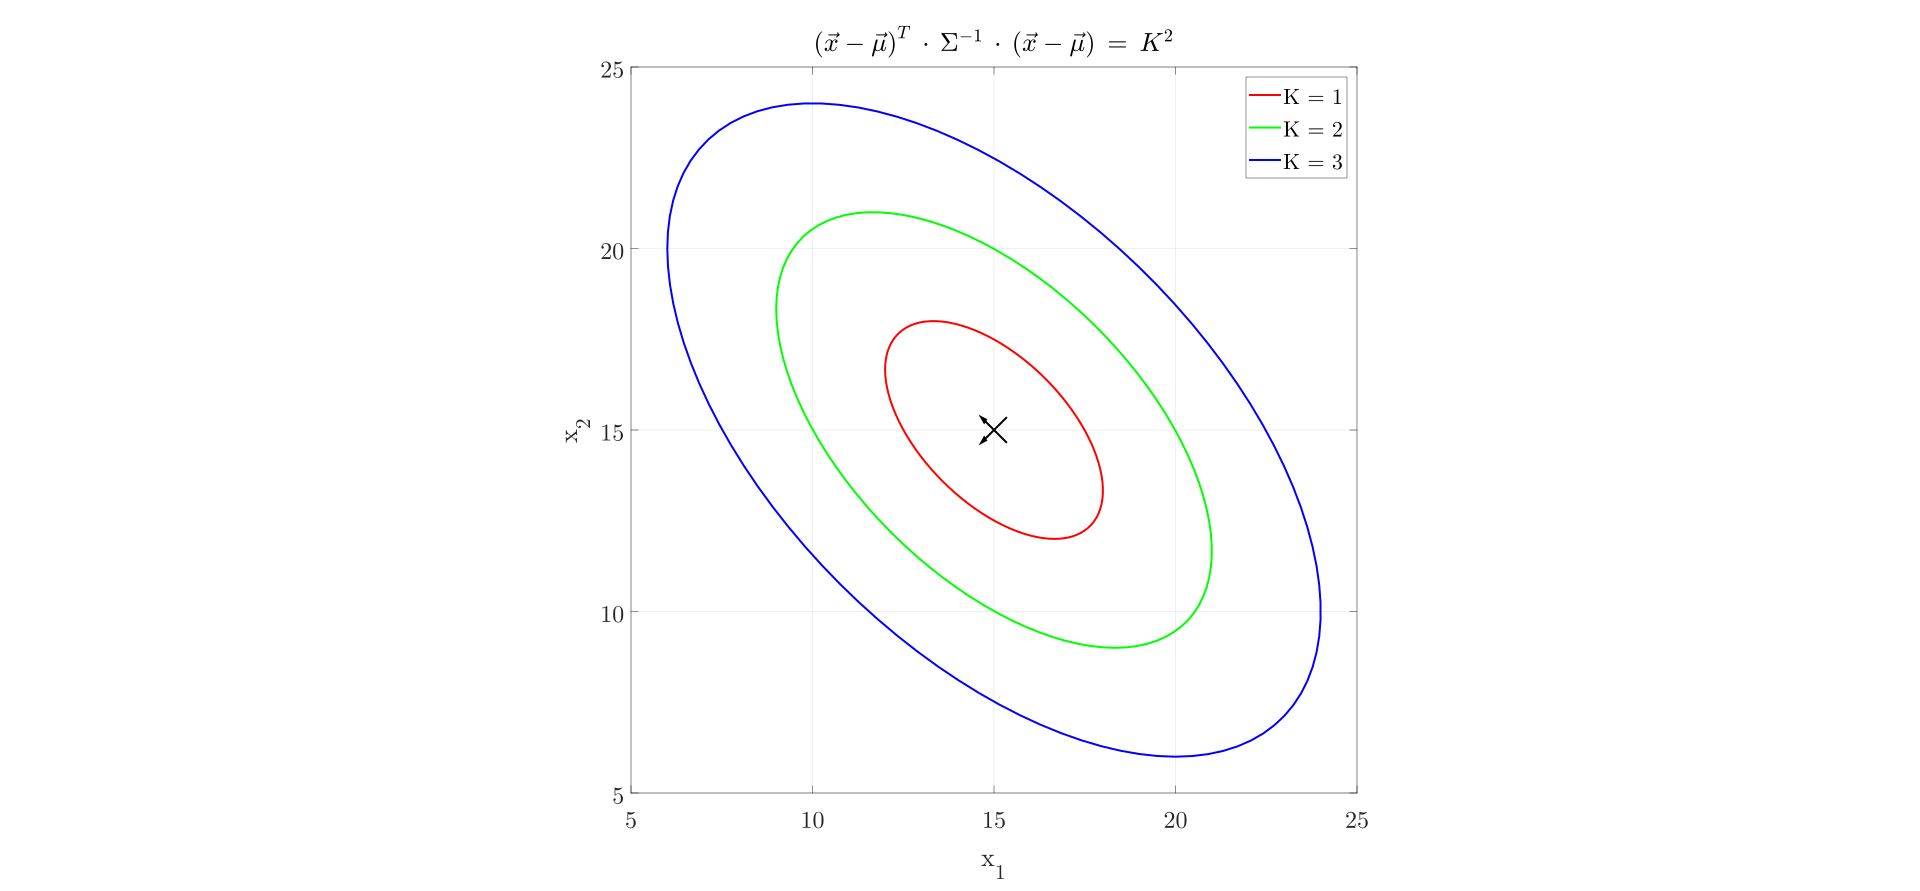
\includegraphics[scale=0.95]{../FIGURES/fig24}
\end{figure}

\begin{align*}
x_t\, &=\, a_t\,\cdot\, x_{t-1}\, +\, b_t\,\cdot\, u_t\, +\,\epsilon_{R_t}\\
\end{align*}

The term$b_t$ is a coefficient that converts from control space to
state space.

The term$\epsilon_{R_t}$ is the system noise:

\begin{align*}
p\left(\epsilon_{R_t}\right)\, &=\,\mathcal{N}\left(0,\,\sigma_{R_t}^2\right)\\
p\left(x_t\, |\, x_{t-1},\, u_t\right)\, &=\,\mathcal{N}\left(\mu_*,\,\sigma_*^2\right)
\end{align*}

\begin{align*}
\mu_*\, =\, E\begin{pmatrix}x_t\, |\, x_{t-1},\, u_t\end{pmatrix}\, &=\, E\begin{pmatrix}a_t\,\cdot\, x_{t-1}\, +\, b_t\,\cdot\, u_t\, +\,\epsilon_{R_t}\, |\, x_{t-1},\, u_t\end{pmatrix}\, =\\
&=\, E\begin{pmatrix}a_t\,\cdot\, x_{t-1}\, |\, x_{t-1}\end{pmatrix}\, +\, E\begin{pmatrix}b\,\cdot\, u_{t}\, |\, u_t\end{pmatrix}\, +\, E\begin{pmatrix}\epsilon_{R_t}\end{pmatrix}\, =\\
&= a_t\,\cdot\, x_{t-1}\, +\, b_t\,\cdot\, u_t
\end{align*}

\begin{align*}
\sigma_*^2\, &=\, E\begin{pmatrix}\left(x_t\, -\, E\begin{pmatrix}x_t\end{pmatrix}\right)^2\, |\, x_{t-1},\, u_t\end{pmatrix}\, =\\
&=\, E\begin{pmatrix}\left(a_t\,\cdot\, x_{t-1}\, +\, b_t\,\cdot\, u_t\, +\,\epsilon_{R_t}\, -\, a_t\,\cdot\, x_{t-1}\, -\, b_t\,\cdot\, u_t\right)^2\, |\, x_{t-1},\, u_t\end{pmatrix}\\
&=\, E\begin{pmatrix}\epsilon_{R_t}^2\end{pmatrix}\, =\,\, E\begin{pmatrix}\left(\epsilon_{R_t}\, -\, 0\right)^2\end{pmatrix}\, =\,\sigma_{R_t}^2
\end{align*}

\begin{align*}
p\left(x_t\, |\, x_{t-1},\, u_t\right)\, &=\,\mathcal{N}\left(\mu_*,\sigma_*^2\right)\\
&=\,\mathcal{N}\left(a_t\,\cdot\, x_{t-1}\, +\, b_t\,\cdot\, u_t,\,\sigma_{R_t}^2\right)
\end{align*}

\begin{align*}
\overline{bel}\left(x_t\right)\, &=\,\int_{x_{t-1} = -\infty}^{+\infty}{p\left(x_t\, |\, x_{t-1},\, u_t\right)\,\cdot\, bel\left(x_{t-1}\right)\,\cdot\, dx_{t-1}}\\
&=\,\int_{x_{t-1} = -\infty}^{\infty}{\mathcal{N}\left(a_t\,\cdot\, x_{t-1}\, +\, b_t\,\cdot\, u_t,\,\sigma_{R_t}^2\right)\,\cdot\,\mathcal{N}\left(\mu_{t-1},\,\sigma_{t-1}^2\right)\,\cdot\, dx_{t-1}}\\
&=\,\gamma\,\cdot\,\int_{x_{t-1} = -\infty}^{+\infty}{e^{-\frac{1}{2}\left(\frac{x_t\, -\,\left(a_t\,\cdot\, x_{t-1}\, + b_t\,\cdot\,\,u_t\right)}{\sigma_{R_t}}\right)^2}\,\cdot\, e^{-\frac{1}{2}\left(\frac{x_{t-1}\, -\,\mu_{t-1}}{\sigma_{t-1}}\right)^2}\,\cdot\, dx_{t-1}}\, =\,\mathcal{N}\left(\overline{\mu_t},\,\overline{\sigma_t}^2\right)\\
\end{align*}
\begin{center}
(More details about this expressions in the book``Probabilistic Robotics''
(Thrun, Burgardm, Fox))
\par\end{center}

\begin{figure}[H]
\centering\includegraphics[scale=1.1]{../FIGURES/fig25}
\end{figure}

\newpage
\begin{center}
\textbf{THE KALMAN FILTER IN 1 DIMENSION}
\par\end{center}
\begin{enumerate}
\item \textbf{PREDICTION:}\\
\textbf{\begin{align*}
x_t\, &=\, a_t\,\cdot\, x_{t-1}\, +\, b_t\,\cdot\, u_t\, +\,\epsilon_{R_t}\\
\end{align*}}The term$\epsilon_{R_t}$ is the system noise:\begin{align*}
p\left(\epsilon_{R_t}\right)\, &=\,\mathcal{N}\left(0,\,\sigma_{R_t}^2\right)\\
\end{align*}\begin{align*}
p\left(x_t\, |\, x_{t-1},\, u_t\right)\, &=\,\mathcal{N}\left(a_t\,\cdot\, x_{t-1}\, +\, b_t\,\cdot\, u_t,\,\sigma_{R_t}^2\right)\\
bel\left(x_{t-1}\right)\, &=\, p\left(x_{t-1}\, |\, z_{t-1}\right)\, =\,\frac{p\left(z_{t-1}\, |\, x_{t-1}\right)\,\cdot\, p\left(x_{t-1}\right)}{p\left(z_{t-1}\right)}\ =\,\alpha\,\cdot\, p\left(z_{t-1}\, |\, x_{t-1}\right)\,\cdot\,\overline{bel}\left(x_{t-1}\right)\, =\\
&=\,\mathcal{N}(\mu_{t-1},\,\sigma_{t-1}^{2})\\
\overline{bel}\left(x_t\right)\, &=\,\int_{x_{t-1} = -\infty}^{+\infty}{p\left(x_t\, |\, x_{t-1},\, u_t\right)\,\cdot\, bel\left(x_{t-1}\right)\,\cdot\, dx_{t-1}}\, =\\
&=\,\int_{x_{t-1} = -\infty}^{+\infty}{\mathcal{N}\left(a_t\,\cdot\, x_{t-1}\, +\, b_t\,\cdot\, u_t,\,\sigma_{R_t}^2\right)\,\cdot\,\mathcal{N}\left(\mu_{t-1},\,\sigma_{t-1}^2\right)\,\cdot\, dx_{t-1}}\, =\,\mathcal{N}\left(\overline{\mu_t},\,\overline{\sigma_t}^{2}\right)
\end{align*}\textbf{\begin{align*}
\overline{\mu_t}\, &=\, a_t\,\cdot\,\mu_{t-1}\, +\, b_t\,\cdot\, u_t\\
\overline{\sigma_t}^2\, &=\, a_t^2\,\cdot\,\sigma_{t-1}^2\, +\,\sigma_{R_t}^2
\end{align*}}
\item \textbf{CORRECTION:}\\
\textbf{\begin{align*}
z_t\, &=\, c_t\,\cdot\, x_t\, +\,\epsilon_{Q_t}
\end{align*}}The term\textbf{$\epsilon_{Q_t}$}is the measurement noise:\\
\begin{align*}
p\left(\epsilon_{Q_t}\right)\, &=\,\mathcal{N}\left(0,\,\sigma_{Q_t}^2\right)
\end{align*}\textbf{\begin{align*}
p\left(z_t\, |\, x_t\right)\, & =\,\mathcal{N}(c_t\,\cdot\, x_t,\,\sigma_{Q_t}^{2})\\
\overline{bel}\left(x_t\right)\, & =\,\mathcal{N}(\overline{\mu_t},\,\overline{\sigma_t}^2)\\
bel\left(x_t\right)\, & =\, p\left(x_t\, |\, z_t\right)\, =\,\alpha\,\cdot\, p\left(z_t\, |\, x_t\right)\,\cdot\,\overline{bel}\left(x_t\right)\, =\\
& =\,\alpha\,\cdot\,\mathcal{N}(c_t\,\cdot\, x_t,\,\sigma_{Q_t}^{2})\,\cdot\,\mathcal{N}(\overline{\mu_t},\,\overline{\sigma_t}^2)\, =\,\mathcal{N}(\mu_t,\,\sigma_t^{2})
\end{align*}\begin{align*}
K_t\, &=\,\frac{c_t\,\cdot\,\overline{\sigma_t}^2}{c_t^2\,\cdot\,\overline{\sigma_t}^2\, +\,\sigma_{Q_t}^2}\\
\mu_t\, &=\,\overline{\mu_t}\, +\, K_t\,\cdot\,\left(z_t\, -\, c_t\,\overline{\mu_t}\right)\\
\sigma_t^2\, &=\,\left(1\, -\, K_t\,\cdot\, c_t\right)\,\cdot\,\overline{\sigma_t}^2
\end{align*}}\\
\begin{align*}
K_t\, &=\, 0\,\,\longrightarrow\,\,\mu_t\, =\,\overline{\mu_t},\,\sigma_t^2\, =\,\overline{\sigma_t}^2\\
K_t\, &>\, 0\,\,\longrightarrow\,\,\sigma_t^2\, <\,\overline{\sigma_t}^2
\end{align*}
\end{enumerate}
\begin{figure}[H]
\centering\includegraphics[scale=0.95]{../FIGURES/fig26}
\end{figure}

\newpage

\begin{figure}[H]
\centering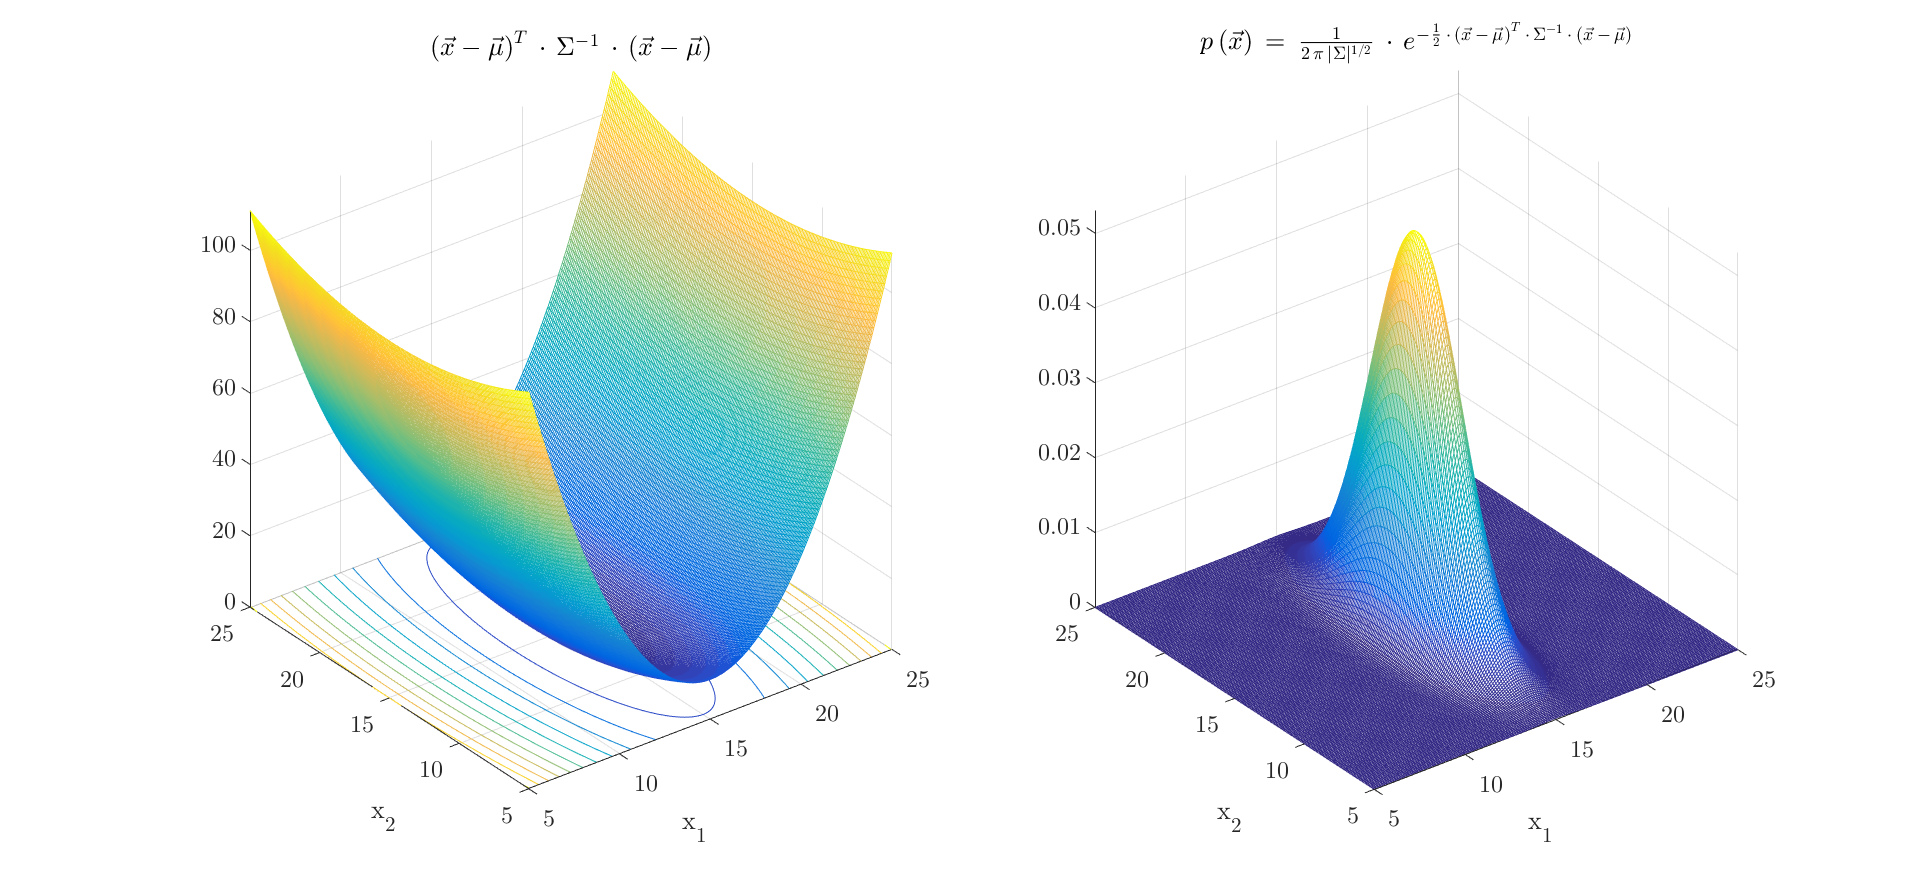
\includegraphics[scale=0.95]{../FIGURES/fig28}
\end{figure}

\end{document}
